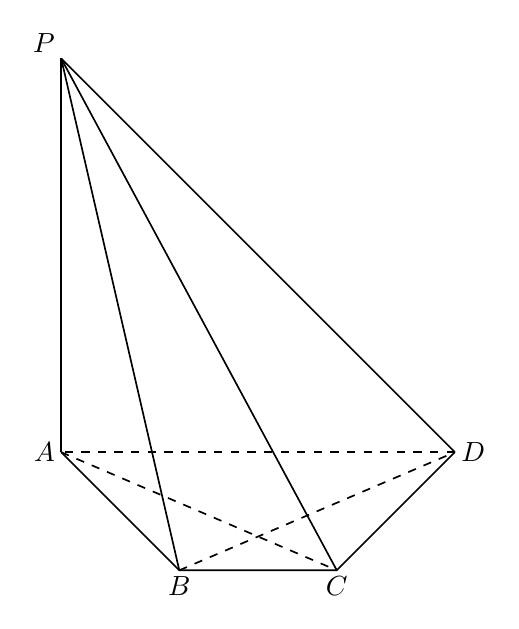
\begin{tikzpicture}[x=1cm,y=1cm,line width=.6pt,font=\normalsize,
geometry edge/.style={solid,line width=.6pt},
geometry label/.style={font=\normalsize,inner sep=2pt}]
\coordinate (P) at (0,7.0);
\coordinate (A) at (0,2.0);
\coordinate (B) at (1.5,0.5);
\coordinate (C) at (3.5,0.5);
\coordinate (D) at (5.0,2.0);
\draw[geometry edge] (P)--(A);
\draw[geometry edge] (P)--(B);
\draw[geometry edge] (P)--(C);
\draw[geometry edge] (P)--(D);
\draw[geometry edge] (A)--(B)--(C)--(D);
\draw[geometry edge,dashed] (D)--(A);
\draw[geometry edge,dashed] (A)--(C);
\draw[geometry edge,dashed] (B)--(D);
\node[geometry label,above left] at (P) {$P$};
\node[geometry label,left] at (A) {$A$};
\node[geometry label,below] at (B) {$B$};
\node[geometry label,below] at (C) {$C$};
\node[geometry label,right] at (D) {$D$};
\end{tikzpicture}
